\documentclass[../main.tex]{subfiles}

\begin{document}

 	\section{Illegale Drogenmärkte}
 	
 	Die meisten psychoaktiven Substanzen werden auf illegalen Märkten, den sogenannten Schwarzmärkten gehandelt.
	Diese Märkte sind vor allem für ihre Kriminalität bekannt, namentlich Gewalt und Korruption. 
	Die theoretische Ökonomie eines allgemeinen Drogenmarktes wird auf den Schweizer Cannabismarkt angewendet.

	
	
	\subsection{Marktteilnehmer}
	Schwarzmärkte unterscheiden sich prinzipiell ökonomisch nicht gross von legalen Märkten.
	Ein Schwarzmarkt verhält sich wie ein freier Markt ohne staatliche Eingriffe, jedoch stehen die Anbieter in einer höheren Position.
	
	
	\subsubsection{Anbieter}	
	Ein Anbieter im Schwarzmarkt nimmt generell immer eine höhere Position als der Nachfrager ein.
	Sie können wie Kartelle oder sogar Monopole handeln und besitzen nahezu uneingeschränkte Macht über die Preisgestaltung.
	Händler können so hohe Margen anstreben und das potentielle Risiko durch einen Risikozuschlag ausgleichen.
	Hohe Margen ziehen alle Arten von Händlern gleichermassen an.
	Kleinere Anbieter werden hingegen zusätzlich aufgrund des Fehlen der Opportunitätskosten zum Markteinstieg bewegt.
	Neben der Preisgestaltung bringt auch das Fehlen der Justiz die Anbieter in eine höhere Position, da sie ohne Rechtsdurchsetzung ihre Forderungen mit Gewalt durchsetzen werden.
	Je höher man in der Lieferkette nach oben wandert, werden die Anbieter professioneller und gewalttätiger. 
	Dies führt dazu, dass man die Annahme tätigen kann, dass der Anbieter dem Nachfrager immer überlegen ist.\\
	
	\noindent
	Marketing gibt es kaum, da die Anbieter möglichst unauffällig agieren wollen.
	Die Kundenbindung erfolgt durch die Kunden, die mittels Mund-zu-Mund Propaganda den Anbietern neue Kunden liefern.
	Auf den ersten Blick existieren nur wenige Anreize für Innovation, da das nachgefragte Produkt in Theorie ziemlich heterogen ist und nur durch den Reinheitsgrad variieren kann.		
	Der grösste Teil der Innovation erfolgt nicht beim Produkt sondern bei den unternehmerischen Prozessen. 
	Eine Erhöhung der repressiven Massnahmen der Polizei kann zur Folge haben, dass Anbieter mehr in Sicherheit und Anonymität investieren.
	Die direkte Folge davon ist, dass der Handel immer professioneller und verdeckter wird. 
	Dieser Effekt wird im Kapitel \texttt{Illegale Drogenmärkte > Preiselastizität} genauer analysiert.
	
	
	\subsubsection{Nachfrager}
	Die Interaktion zwischen Nachfrager und Anbieter basiert hauptsächlich auf Vertrauen.
	Gesetze können nicht auf das Handeln auf dem Markt angewendet werden, da beide Parteien illegal handeln und keine Partei eine Strafverfolgung riskieren will.
	Für Nachfrager existiert keine Sicherheit auf Qualität, Quantität und Verfügbarkeit der Güter.
	Sie können Opfer von Betrug aber auch Gewalttaten werden, ohne dass sie sich wehren können.\\
	
	\noindent	
	Die Endkonsumenten, ein Teil der Nachfrager werden noch stärker als Händler, die als Nachfrager agieren, benachteiligt.
	Da Cannabis auch zu den suchterzeugenen Substanzen gezählt werden kann, werden die Prävalenzen der Konsumenten immer weiter steigen.
	Dies hat zur Folge, dass die Ausgaben der Konsumenten immer weiter steigen, bis sie nicht mehr in der Lage ihren Konsum zu finanzieren.
	Vielen Menschen bleiben in so einer Situation keine Opportunitätskosten mehr übrig, weswegen sie in die Beschaffungskriminalität abrutschen.
	
	
	\subsubsection{Staat}
	Der Staat nimmt eine passive Position im Markt ein und ist kein direkter Marktteilnehmer, versucht aber mit Gegenmassnahmen entgegenzuwirken.
	Während früher das einzige Mittel die vollständige Marktregulierung durch Repression war, werden heute nicht nur repressive Massnahmen getätigt.
	Die Vier-Säulen-Politik ist das wichtigste Mittel der Schweizer Drogenpolitk. 
	In 4 verschiedenen Bereichen werden Massnahmen getätigt, so dass das Schadensausmass des Drogenkonsums und Drogenhandels möglichst gering gehalten wird.
	Diese Politik ist in \texttt{Art. 1a BetmG} seit der Revision des Betäubungsmittelgesetzes ein fester Bestandteil der Drogenpolitik.
	Die vier verschiedenen Bereiche sind:
	\begin{singlespacing}
	\begin{enumerate}
		\item Prävention
		\item Therapie und Wiedereingliederung
		\item Schadensminderung und Überlebenshilfe
		\item Kontrolle und Repression
	\end{enumerate}
	\end{singlespacing}    
    
	\noindent
	Das seit 2016 bewährte Vier-Säulen-Modell wurde mit vier weiteren Handlungsfeldern erweitert. 
	Die Stategie wird vom Bundesamt für Gesundheit (BAG) festgelegt und in einem Bericht der Öffentlichkeit mitgeteilt \cite{bag-2015}.	
	Neben den vier Hauptaufgaben wurden vier weitere Querschnittsaufgaben hinzugefügt.
	Die vier zusätzlichen Handlungsfelder dienen zur Steuerung und Koordination.
	Namentlich heissen die Felder "Koordination und Kooperation", "Wissen", "Sensibilisierung und Information" und "Internationale Politik".

	\noindent
	{
		\centering
		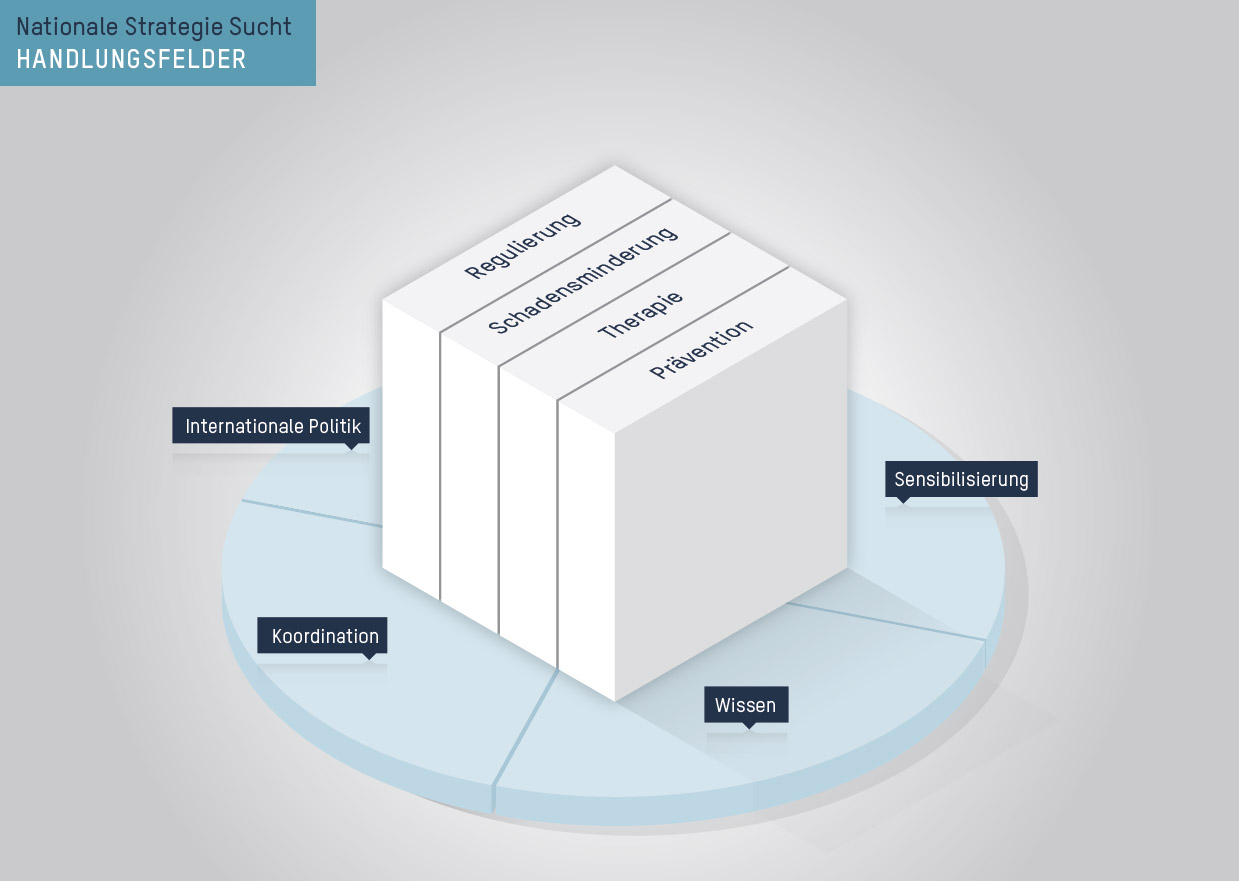
\includegraphics[width=0.8\linewidth]{VSP-erweitert}
		\captionsetup{font=small}
		\captionof{figure}{Erweiterung der Viersäulenpolitik}
		\small 
		\noindent
		\begin{center}
		Quelle: \cite{bag-2015}
		\end{center}
	}
	
	\noindent
	Die Viersäulenpolitik der Schweiz konnte sich schon mehrfach beweisen.
	Als gutes Beispiel dient die Krise am Platzspitz, als im Jahre 1986 das Verbot für die Spritzenabgabe aufgehoben wurde und die Anzahl der Drogentoten sank.
	Die Präventionsarbeit in den Schulen trägt dazu bei, dass ein generelles Verständnis in der Gesellschaft vorhanden ist.
	
	\subsection{Preiselastizität}
	Die Preiselastizität zeigt an, wie stark das Angebot oder die Nachfrage auf eine Preisänderung reagiert.
	Bei Cannabis wird die Preiselastizität der Nachfrage wie bei vielen Suchtmitteln sehr unelastisch eingeschätzt $(-1<\varepsilon_{xy}<0)$. 
	Nach einer Studie beträgt der Wert für die Preiselastizität der Nachfrage -0.54\% \cite{golzar}.
	Die Preiselastizität von -0.54 ist der direkte Auslöser, dass eine Preiserhöhung von 1\% einen Nachfragerückgang von 0.54\% zur Folge hat.\\
	
	\noindent
	Eine Prohibition wirkt aufgrund der unelastischen Nachfragekurve nicht positiv ein.
	Eine Verschärfung der Strafverfolgung der Händler und Produzenten bewirkt keinen grossen Rückgang der Nachfrage, jedoch eine Erhöhung des Preises.
	Die Händler schlagen auf ihre Preise einen Risikozuschlag auf und wälzen diesen an ihre Kunden ab.
	Da die Konsumenten aufgrund ihrer Sucht jedoch nicht auf ihr Gut verzichten können, sinkt die Nachfrage kaum.\\
	
	%\noindent
	%{
	%	\centering
	%	\includegraphics[width=0.8\linewidth]{example-image-a}
	%	\captionsetup{font=small}
	%	\captionof{figure}{Preiselastizität}
	%	\small 
	%	\noindent
	%	\begin{center}
	%	Quelle: Eigene Darstellung
	%	\end{center}
	%}
	
	\noindent
	Dieser Effekt wurde bereits analysiert und nennt man "rational addiction" \cite{becker}.
	Aus ökonomischer Sicht bringt die Prohibition nur bedingt einen Erfolg in der Bekämpfung des Drogenkonsums. 
	Auf den ersten Blick scheint sie die gewünschte Wirkung zu zeigen, jedoch entsteht dadurch ein anderer Nebeneffekt. 
	Dadurch dass die Preise steigen und die Nachfrage kaum zurückgehen kann, sind die Konsumenten gezwungen die hohen Geldsummen zu bezahlen.
	Dies führt zu einer erhöhten Beschaffungskriminalität der unteren Gesellschaftsschicht, somit ergibt sich eine erhöhte Kriminalität. 
	Eine erhöhte Kriminalität liegt nicht im Interesse der Allgemeinheit und steht somit dem Grundsatz des öffentlichen Interesses entgegen.
	

	
	\subsection{Sozioökonomie}
	
	\paragraph{Datenbasis}
	Als Datenbasis dient eine Umfrage vom Suchtmonitoring Schweiz \cite{gmel}.
	Die Prävalenz gibt an, wieviele Konsumenten in einem gewissen Zeitbereich Cannabis konsumiert haben.
	Die Lebenszeitprävalenz stellt dar, wie viele Schweizer mindestens einmal in ihrem Leben Cannabis konsumiert haben.
	Diese Regel gilt nach gleichem Prinzip für die 12-Monatsprävalenz und die 30-Tagesprävalenz.
	
	\paragraph{Prävalenz}	
	Gemäss einer Befragung des Suchtmonitoring haben $33.8\%$ der Schweizer Bevölkerung schon einmal in ihrem Leben Cannabis konsumiert.
	Die Tendenz ist seit Jahren leicht steigend und scheint auch kein Ende zu nehmen. 
	So stieg die Lebenszeitprävalenz in 5 Jahren (2011 bis 2016) um 5 Prozentpunkte. 
	Der Konsum ist in allen Altersklassen präsent und es herrscht keine generelle Abneigung gegenüber dem Konsum. 
	Es zeichnet sich klar ab, dass vor allem jüngere Leute Cannabis konsumieren. 
	Bei der jüngeren Bevölkerung von 20-34 Jahren ist es sogar die Mehrheit, die mindestens einmal in ihrem Leben Cannabis konsumiert hat.\\
	
	\noindent
	{
		\centering
		\includegraphics[width=\linewidth]{LebenszeitprävalenzGmel}
		\captionsetup{font=small}
		\captionof{figure}{Lebenszeitprävalenz}
		\small 
		\noindent
		\begin{center}
		Quelle: \cite{gmel}
		\end{center}
	}
	
	\noindent
	Die 12-Monatsprävalenz ist von $5.0\%$ auf $7.3\%$ gestiegen, während die 30-Tagesprävalenz keinen grossen Anstieg aufzeigt. 
	Anhand dem Verhältnis der beiden Prävalenzen kann man erkennen, dass der chonische Konsum kaum angestiegen ist, jedoch die Bereitschaft zum Probekonsum gestiegen ist. 
	Man kann annehmen, dass der Probierkonsum weiterhin ansteigen wird und sich dies in Zukunft in der Lebenszeitprävalenz zeigen wird.
	Die Entwicklung verrät auch, dass die Gesellschaft den Konsum nicht mehr stigmatisiert, auch wenn sie nicht regelmässig konsumiert.\\
	
	\noindent
	{
		\centering
		\includegraphics[width=\linewidth]{KurzzeitprävalenzGmel}
		\captionsetup{font=small}
		\captionof{figure}{12-Monats- und 30-Tageprävalenz}
		\small 
		\noindent
		\begin{center}
		Quelle: \cite{gmel}
		\end{center}
	}
	
	\paragraph{Vergleich}
	Im Vergleich zu anderen illegalen Drogen hat Cannabis einen grossen Vorsprung.
	Die Lebenszeitprävalenz von den zwei nächsthöchten Substanzen sind wesentlich kleiner.
	Es konsumierten im Jahr 2016 4.2\% aller Schweizer mindestens einmal in ihrem Leben Kokain und 3.9\% Ecstasy.
	Der fast achtfache Unterschied lässt darauf schliessen, dass man Cannabis nicht gleich behandeln kann wie andere illegale Substanzen. 
	% TODO: Abbildung Vergleich
	
	\paragraph{Schlussfolgerung}
	Aus den Daten erkennt man, dass Cannabis einen anderen Stellenwert in der Gesellschaft hat wie andere illegale Drogen.
	Der Konsum ist mittlerweile weit verbreitet und wird auch von der Mehrheit akzeptiert.
	Dies ist eine Voraussetzung, dass man überhaupt eine Legalisierung in Betracht ziehen kann.
	Das Verbot scheint nicht die gewünschte Wirkung zu zeigen und die Entwicklung zeigt, dass immer weniger Schweizer das Gesetz beachten.
	Das Ziel der Prohibition ist es, den Konsum der Bevölkerung zu senken, jedoch steigen die Prävalenzen seit der Einführung der Prohibition.
	Da die repressiven Massnahmen nicht funktionieren, müsste man untersuchen, ob und wie man mit einer Legalisierung dennoch die kurzzeitigen Prävalenzen tief halten kann.
	
	
	\subsection{Ökonomie}
	
	\paragraph{Preis}
	Der durchschnittliche Preis für Cannabis befindet sich bei CHF 10.-, während der Preis von Haschisch mit CHF 13.- etwas höher liegt \cite{zobel}.
	Den erhöhten Preis von Haschisch kann man so erklären, dass die Wirkung meistens viel potenter ausfällt und die Herstellung aufwendiger ist.
	Haschisch stellt im Gegensatz zu Cannabis ein konzentriertes THC Produkt dar.
	Der Preis wurde durch den Risikozuschlag und den hohen Margen in die Höhe getrieben.
	Der eigentliche Marktpreis von THC haltigem Cannabis liegt weitaus tiefer.
	
	
	\paragraph{Marktvolumen}
	Alleine im Kanton Waadt werden pro Jahr 3.5 bis 5.1 Tonnen Cannabis konsumiert \cite{zobel}. 	
	Wenn man das Marktvolumen vom Kanton Waadt auf die ganze Schweiz linear hochrechnet, kommt man auf ein gesamtschweizerisches Marktvolumen von 37.5-54.7 Tonnen.
	Das Marktvolumen gibt ungefähr die Grössenordnung an, wird jedoch leicht kleiner sein, da der Konsum im Kanton Waadt höher ist im Vergleich zu anderen Kantonen.
	\\
	
	\noindent
	Der Markt an THC-Produkten besteht aus zwei grossen Teilen, dem Markt von Cannabis und dem von Haschisch.
	Etwa 70\% der Produkte bestehen aus Cannabis während die restlichen 30\% Haschisch sind.
	Anteile anderer Produkte sind vernachlässigbar, da kein richtiger Markt existiert oder die Anteile zu klein sind.
	Beide Produkte sind in der Wirkung recht ähnlich, da bei beiden der Inhaltsstoff THC vorhanden ist.
	In dieser Arbeit wird nur Cannabis erwähnt, jedoch sind damit immer beide Substanzen gemeint.
	
	\paragraph{Entwicklung}
	Die Produkte können sich nur durch den THC Gehalt unterscheiden.
	In dieser Arbeit werden beide Produkte, Cannabis und Haschisch, als heterogene Güter betrachtet.
	Teilweise schwankt zwar die Qualität von Region zu Region, jedoch sind die meisten Produkten frei von Streckmitteln.
	Der THC Gehalt von Cannabis blieb in den letzten 10 Jahren immer stabil.
	Bei Haschisch ist der THC Gehalt seit dem Jahr 2007 konstant am steigen.
	So stieg er von 10.4\% auf 22.0\% in nur 12 Jahren \cite{sgrm}.
	Auch in Zukunft wird dieser Anteil immer weiter steigen, was sich auf die Konsumenten nicht positiv auswirken wird, da das Produkt so schwerer zu dosieren ist.
	
	\noindent
	{
		\centering
		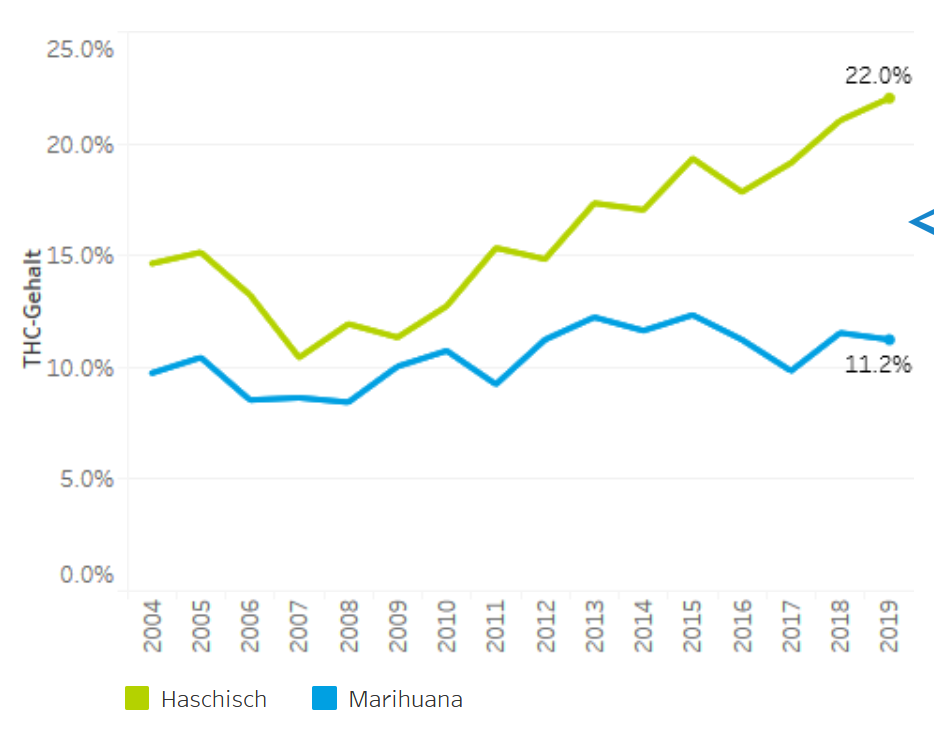
\includegraphics[height=10cm]{THCGehalt}
		\captionsetup{font=small}
		\captionof{figure}{Entwicklung des THC Gehalts}
		\small 
		\noindent
		\begin{center}
		Quelle: \cite{sgrm}
		\end{center}
	}	
	
\end{document}